% Chapter 1

\chapter{Introducción general} % Main chapter title

\label{Chapter1} % For referencing the chapter elsewhere, use \ref{Chapter1} 
\label{IntroGeneral}

%----------------------------------------------------------------------------------------

% Define some commands to keep the formatting separated from the content 
\newcommand{\keyword}[1]{\textbf{#1}}
\newcommand{\tabhead}[1]{\textbf{#1}}
\newcommand{\code}[1]{\texttt{#1}}
\newcommand{\file}[1]{\texttt{\bfseries#1}}
\newcommand{\option}[1]{\texttt{\itshape#1}}
\newcommand{\grados}{$^{\circ}$}

%----------------------------------------------------------------------------------------

%\section{Introducción}

%----------------------------------------------------------------------------------------
\section{Hogares inteligentes}

La domótica es la aplicación de la tecnología a la automatización del hogar, que se utiliza para controlar y gestionar diferentes sistemas y dispositivos, con el fin de aportar seguridad, bienestar y confort. Estos sistemas pueden abarcar la iluminación, la calefacción, el aire acondicionado, los sistemas de seguridad y cámaras de vigilancia, los sistemas de entretenimiento y otros dispositivos domésticos \citep{1}.

Este sector, como muchos otros que utilizan tecnología ha estado creciendo, al punto que algunas de las viviendas modernas son concebidas como hogares inteligentes desde su edificación, llegando a tener edificios completos con este tipo de soluciones instaladas.

\subsection{Aplicaciones comunes}

Los servicios que ofrece la domótica se pueden agrupar según cinco aspectos o ámbitos principales \citep{2}:

\begin{itemize}
	\item Programación y ahorro energético: el ahorro energético no es algo tangible, sino legible con un concepto al que se puede llegar de muchas maneras. En muchos casos no es necesario sustituir los aparatos o sistemas del hogar por otros que consuman menos energía sino una gestión eficiente de los mismos.
	\item Confort: conlleva todas las actuaciones que se puedan llevar a cabo que mejoren la comodidad en una vivienda. Dichas actuaciones pueden ser de carácter tanto pasivo, como activo o mixtas.
	\item Seguridad: consiste en una red encargada de proteger tanto los bienes patrimoniales, como la seguridad personal y la vida.
	\item Comunicaciones: son los sistemas o infraestructuras de comunicaciones que posee el hogar.
	\item Accesibilidad: bajo este mecanismo se incluyen las aplicaciones o instalaciones de control remoto del entorno que favorecen la autonomía personal de personas con limitaciones funcionales, o discapacidad.
\end{itemize}

El presente trabajo puede encuadrarse dentro de la programación y ahorro energético, confort y accesibilidad. En la figura \ref{fig:2} puede verse una imagen con los distintos tipos de dispositivos que pueden estar conectados a un sistema de domótica.

\begin{figure}[h]
\centering
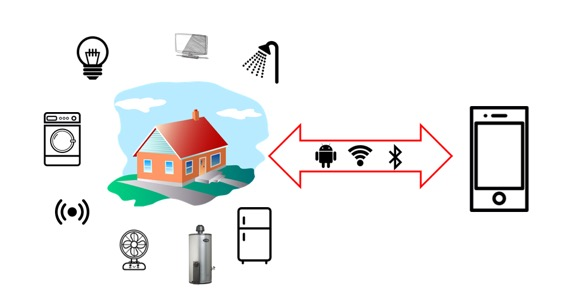
\includegraphics[scale=0.55]{Figura 2 - Domotica.jpg}
\caption[Ejemplo de sistema de domótica]{Ejemplo de sistema de domótica. \protect\footnotemark}
\label{fig:2}
\end{figure}
\footnotetext{Imagen tomada de: \url{https://intelligy.com/blog/2018/03/12/conoces-la-domotica/}}

\section{Motivación}

El uso de la tecnología para facilitar y mejorar la vida de las personas se está implementando en todo el mundo en diversos ámbitos, creando soluciones complejas e innovadoras. Los electrodomésticos e instalaciones se fabrican con posibilidades de conexión y capacidades cada vez más amplias, abarcando funcionalidades complejas que aportan al bienestar y confort de las personas.

Este proyecto nace como mejora y actualización de la tesis de grado de ingeniería, en la cual se creó un sistema similar que carecía de conectividad a Internet y utilizando tecnología que al día de hoy es obsoleta. Es por este motivo que se ha decidido hacer un proyecto académico con esta temática, pudiendo crear un sistema integral con una página web, base de datos que almacene mediciones y utilizando hardware actualizado.

\section{Estado del arte}

En el mercado actual existe una gran cantidad de sistemas de domótica, algunos privados o bajo licencias propietarias y otros con licencias de código abierto, nacionales e internacionales. Aquellas soluciones de código abierto tienen los repositorios públicos en GitHub al alcance de todos para ser descargados, implementados y hasta modificados.

Del mercado internacional, podemos nombrar 2 importantes variantes:
\begin{itemize}
	\item Matter: es un estándar de conectividad de código abierto creado por la \textit{Connectivity standards alliance}. Es de los más importantes a nivel global y participan empresas como Amazon, Apple, Google, Huawei entre muchas otras. Ha crecido y tomado mucha fuerza durante el corto tiempo de vida que tiene el proyecto \citep{3}.
	\item Home assistant: software de automatización de hogares de código abierto que prioriza el control local y la privacidad. Desarrollado por una comunidad mundial de entusiastas de autodidactas y profesionales con un sentido propio \citep{4}.
\end{itemize}

En la figura \ref{fig:3} se observa un kit de Matter a la izquierda y la pantalla de la aplicación de Home Assistant a la derecha.

\begin{figure}[h]
\centering
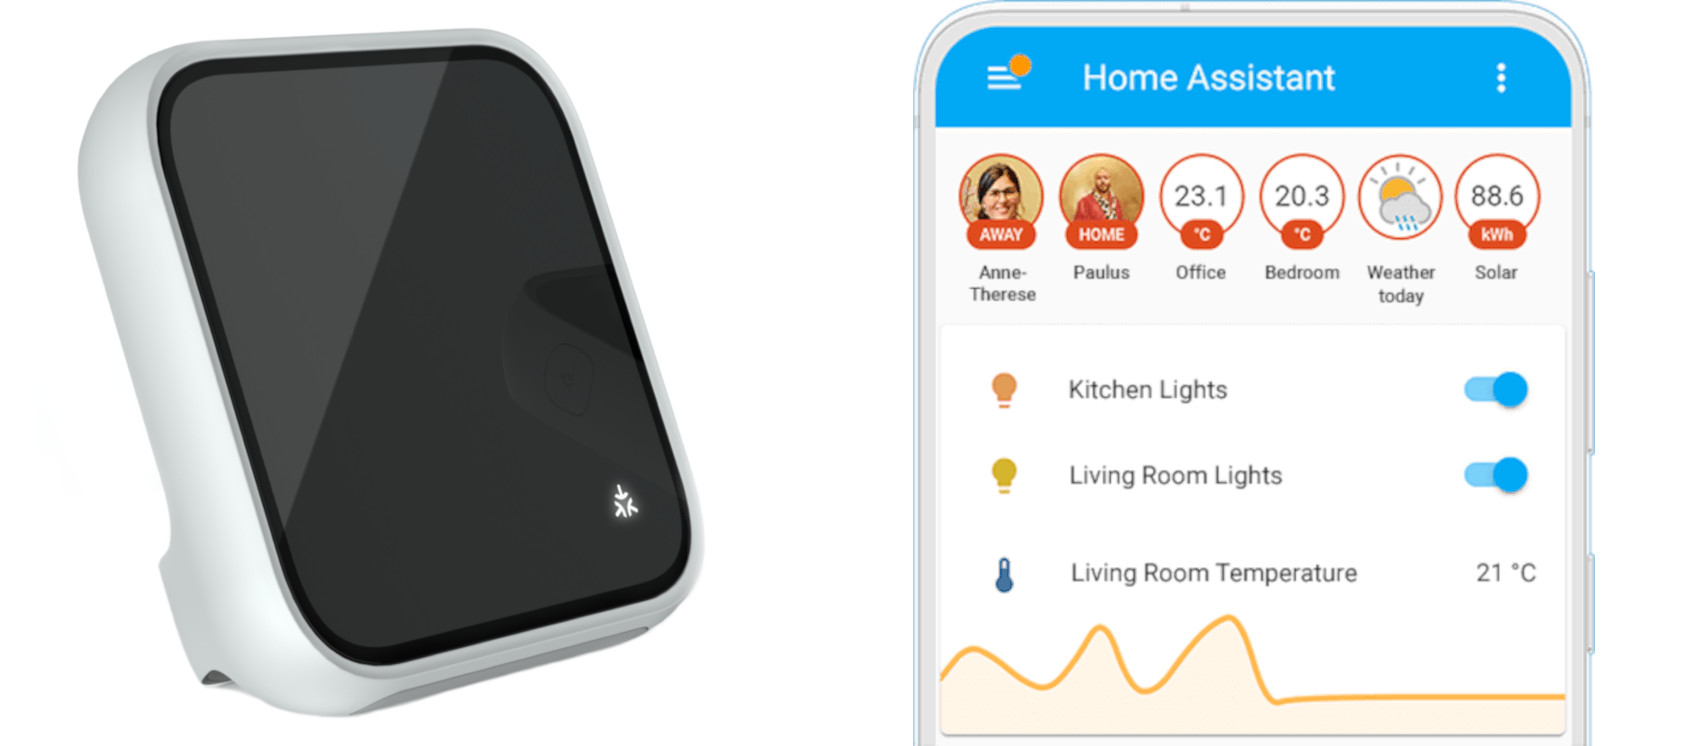
\includegraphics[scale=0.15]{Figura 3 - Soluciones.jpg}
\caption[Matter y Home Assistant]{Matter y Home Assistant. \protect\footnotemark}
\label{fig:3}
\end{figure}
\footnotetext{Imágenes tomadas de: \url{https://csa-iot.org/} y \url{https://www.home-assistant.io/}}

A nivel nacional, existen empresas que se dedican al desarrollo de sistemas de domótica de forma privada:
\begin{itemize}
	\item Domotic \citep{5}.
	\item Commax \citep{6}.
	\item Reactor \citep{7}.
\end{itemize}

Todos estos sistemas utilizan distintos tipos de conexión como Zigbee o Wi-Fi, mensajes entre dispositivos como HTTP, MQTT y otros, y pueden alojar sus plataformas en un servidor local o en la nube.

Sin embargo, pocos de estos sistemas tienen la posibilidad de funcionar con mandos desde el lugar o sin conexión con el servidor, es decir, que sean independientes y controlables de forma local. Este proyecto tiene tal posibilidad, ya que la página web es una forma más de cambiar los parámetros de los nodos y está diseñado para decidir si cada terminal posee comandos o no.

En la tabla \ref{tab:empresas} pueden verse las principales características de las empresas nacionales con soluciones similares.

\begin{table}[h]
\centering
\caption[Comparativa entre las distintas opciones del mercado nacional]{Comparativa entre las distintas opciones.}
\begin{tabular}{l c c}
\toprule
\textbf{Empresa} & \textbf{Productos} & \textbf{Compatibilidad}\\
\midrule
Domotic	& Catálogo amplio & No especifica \\
Commax	& Catálogo amplio & \textit{Smart things} y \textit{Apple Home Kit}	\\
Reactor	& 2 alternativas & \textit{Google Assistant} e \textit{IFTTT} \\
\bottomrule
\hline
\end{tabular}
\label{tab:empresas}
\end{table}

\section{Objetivos y alcance}

El objetivo de este trabajo es aplicar todos los conocimientos adquiridos a lo largo del posgrado en un área de interés particular, que es la domótica. En especial, el principal propósito es desarrollar un prototipo que sirva como punto de partida para un sistema más amplio y avanzado, con la particularidad de que en un futuro cercano se pueda llegar a analizar la opción de integrarlo con sistemas como \textit{Matter} o \textit{Home Assistant}.

En este desarrollo se incluyó:
\begin{itemize}
	\item El esquema de conexiones de las placas de ESP32 con los módulos de display, encoder, driver LED y driver de calefacción.
	\item El diseño en una placa de desarrollo del circuito del driver de corriente continua de la iluminación LED.
	\item El diseño en una placa de desarrollo del circuito del driver de corriente alterna de la calefacción.
	\item La programación de un firmware de la placa ESP32 para la comunicación y manejo de conexiones.
	\item La creación del software frontend, backend y la base de datos que almacena toda la información dentro del servidor.
	\item Las conexiones, instalación y configuración del servidor montado en una Raspberry Pi.
\end{itemize}

En la figura \ref{fig:4} se puede ver un esquema básico del sistema desarrollado.
\begin{figure}[h]
\centering
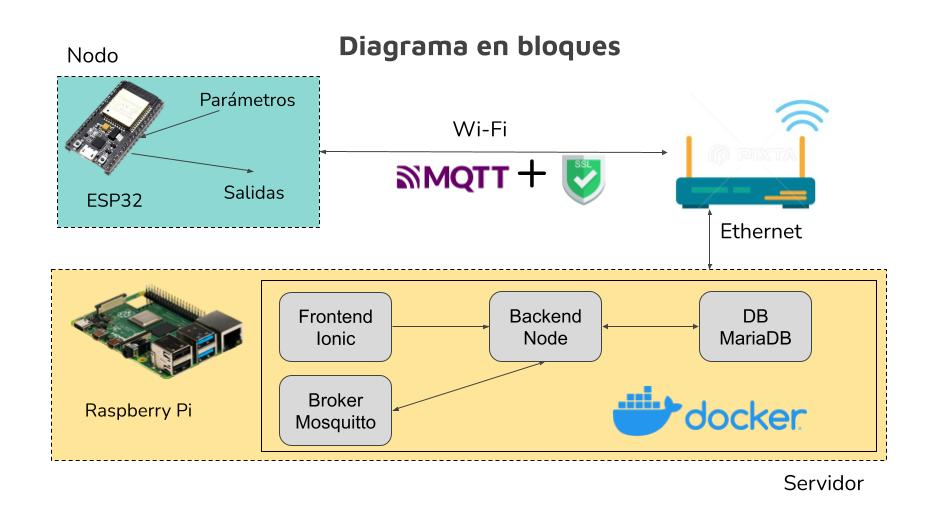
\includegraphics[scale=0.4]{Figura 4 - Diagrama en bloques.jpg}
\caption[Esquema básico del sistema desarrollado]{Esquema básico del sistema desarrollado. \protect}
\label{fig:4}
\end{figure}